\documentclass{acmsiggraph}

\usepackage{parskip}
\usepackage{graphicx}
\usepackage{courier}
\usepackage{footmisc}
\usepackage{listings}
\usepackage{amsmath}
\usepackage{url}
\usepackage{color}
\usepackage{xcolor}
\onlineid{0}

\title{Cinematic Particle Systems with OpenCL}

\author{Tim Horton\thanks{e-mail: hortot2@rpi.edu}\\Rensselaer Polytechnic Institute}

\begin{document}

\maketitle

\begin{figure}
    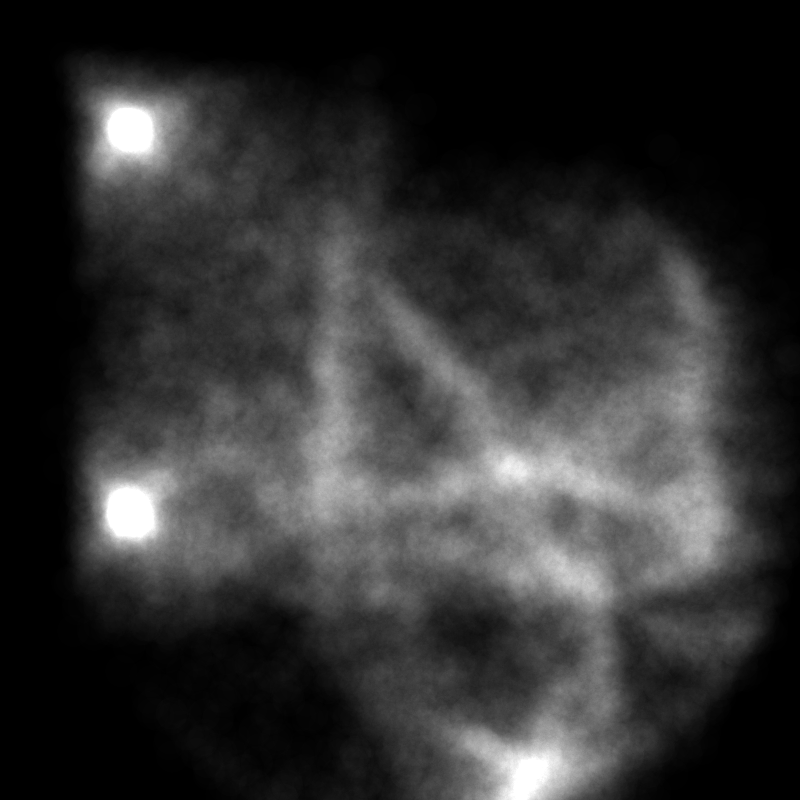
\includegraphics[width=84.5mm]{gravity.png}
    \caption{A simple gravity simulation with two emitters and three supermassive particles (approx. 45,000 particles)}
    \label{titlefig}
\end{figure}

\section*{Abstract}

High-particle-count simulations are becoming increasingly crucial in many different aspects of our world today: both in entertainment --- within video games, movies, and the like --- and in scientific fields, where particle systems are capable of simulating and visualizing many interesting phenomena.

This paper will explore the possibility of parallelizing the simulation of these large particle systems and offloading them to very-parallel\footnote{As opposed to {\it massively-}parallel, like the CCNI's Blue Gene/L, or the {\it slightly}-parallel CPU in most modern computers} hardware which is usually only used for {\it rendering}: the video card.

We will also touch briefly on ways to design a system for describing particle systems in a generalized way, though the majority of the work that is currently in a functional state centers around simulation and rendering.

\section{Introduction}

Simulation of large particle systems requires a large amount of computation --- each particle must be inspected and updated. For certain types of particle systems --- n-body gravity, for example --- each particle is affected by its neighbors, increasing the required calculation time drastically.

This is what we aim to address with this paper. While it's unlikely that we can contribute any improved simulation algorithms, we can instead work to parallelize these algorithms and implement them with OpenCL, which will allow them to run on the GPU contained within modern graphics cards. This paper will demonstrate both the parallelization of the application of forces on large numbers of particles and the significant performance gained by doing so.

We will also explore a simple parallelized particle renderer, as well as the potential for the integration of our simulator into the popular open-source 3D package, Blender.

It is important to understand that the system we've developed is purely for offline work --- it is not suitable for realtime simulation and rendering. Thus, {\it cinematic}. This is primarily because of the relatively poor performance of the renderer. However, as you'll notice in section \ref{performanceSection}, the speedup provided by our work {\it is} actually sufficient to make some simulations fast enough to run in real time, if one were to find a faster renderer.

\section{Prior Art}

\cite{1281670} discusses a system quite similar to ours --- they use the GPU to simulate large-particle-count systems, including computationally-intensive forces like n-body gravity --- however, they make one simplification which drastically improves performance: they assume that the particle data never needs to return to the CPU. This means that the extremely expensive copying to and from video memory which is done continually within our system is completely unnecessary, but also removes the ability to use the particle data in any flexible way (i.e. copying it to a file to be rendered later, etc.).

\section{Implementation}

The code for this paper is available under the two-clause BSD license at:

\url{http://github.com/hortont424/particles}

It consists of about 3000 lines\footnote{According to {\it sloccount}} of C and Objective C, which encompass the curve editor and other design tools, an abstraction layer on top of OpenCL\footnote{the Open Computing Language, a framework for creating programs using a language similar to GLSL and run on the GPU}, and all of the code to drive simulation, preview, and rendering. In addition, there are about 350 {\bf [UPDATE THIS]} lines of OpenCL Kernel Language, which includes the code to apply each of the forces as well as the renderer.

\subsection{Particle Systems}

A particle system is defined by a simple JSON\footnote{JavaScript Object Notation, a format often used today for information exchange in place of things like XML, due to its lightweight nature} file (figure \ref{curveListing} is a very simple example of such a file), which lays out all of the system's parameters: the number of particles to start out with, the location and properties of emitters, the location and properties of forces, and many other things. If {\it Interpolator} had been finished, this file would also contain the mappings between these properties and various curve files.

\begin{figure}

    \lstset{language=Python}
    \lstset{basicstyle=\footnotesize\ttfamily}
    \lstset{stringstyle=\color{blue}\ttfamily}
    \lstset{numbers=left, numberstyle=\tiny, stepnumber=1, numbersep=5pt}
    \begin{lstlisting}[frame=trbl]{}
{
    "initialParticles": {
        "count": 1
    },
    "forces": [
        {
            "kernel": "gravity",
            "strength": 1.0,
            "noise": 0.0,
            "mass": 100000000000.0,
            "particle": {
                "fixed": true,
                "x": 1.2,
                "y": 1.2,
                "z": 0.5
            }
        }
    ],
    "emitters": [
    {
        "birthRate": 20.0,
        "initialVelocity": 0.0,
        "particle": {
            "fixed": true,
            "x": -1.2,
            "y": 1.2,
            "z": 1.5
        }
    }],
    "integration": {
        "kernel": "verlet",
        "timestep": 0.005
    }
}
    \end{lstlisting}

    \caption{A simple sample curve file, with one emitter and one force}
    \label{curveListing}
\end{figure}

\subsection{Design}

\begin{figure}
    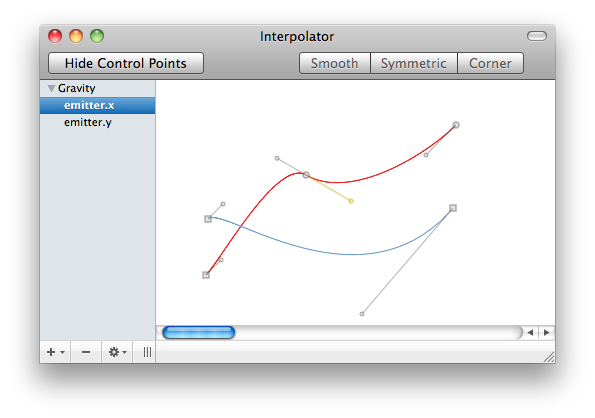
\includegraphics[width=84.5mm]{interpolator.png}
    \caption{A screenshot of the unfinished {\it Interpolator} particle system design tool}
    \label{fig:interpolator}
\end{figure}

The particle system design tools implemented during the course of this project are not entirely functional, as they took a backseat to the simulation, preview, and rendering components, mostly due to the fact that it's possible to design a system by hand.

The primary design tool, which can be seen in figure \ref{fig:interpolator}, is called {\it Interpolator}, as it is quite literally a tool to design interpolation curves. It's a Cocoa application which provides an interface to edit arbitrary B\'{e}zier splines and map them to properties of an element in the particle system. For example, one curve might dictate the $x$ position of an emitter, while another might be mapped to the lifetime that emitter's children.

Since this tool was not finished in time for this paper, it is not integrated into the simulation and rendering phases introduced here.

\subsection{Simulation}

The simulation phase is the heart of our project. Starting from a system description file (as shown in figure \ref{curveListing}), it eventually provides the position of each particle to either the previewing or rendering subsystems in a frame-by-frame manner. It involves various steps, which we'll outline below.

\subsubsection{Parsing the .psys}

The particle system description file, in JSON format, is parsed with Michael Clark's MIT-licensed {\bf json-c} library. All of the properties are read into internal data structures and validated, with reasonable defaults being filled in for missing values.

\subsubsection{Load necessary kernels}

There are quite a few OpenCL kernels included with this project; since the program now knows which ones it needs, it can now instantiate one kernel for each force, as well as one copy of the interpolator kernel.

This is done by making a copy of the appropriate master kernel, all of which are loaded into a kernel library and compiled at the beginning of the process.

\subsubsection{Randomly generate default particles}

Some particle systems have an initial set of particles --- some, because they don't include any emitters, others, because they simply want to start with some particles displayed. At the moment, the only parameter of the initial particles that can be controlled is the number; they are placed randomly in the unit cube with zero initial velocity. Eventually, it would be ideal to support manipulation of the range and location of random positions, as well as of the mass and initial velocity.

\subsubsection{Evaluate emitters}

\label{emitters}

Evaluation of emitters primarily involves adding new particles at the location of the particle and giving them an initial velocity (depending on the emitter's settings).

Emitters are evaluated on the CPU (instead of the GPU). This is done primarily because of a limitation in OpenCL where one cannot resize a buffer from inside a kernel --- so, there would be no way to allocate space from inside an emitter kernel.

One key performance consideration while evaluating emitters is how many new particles to allocate space for. If we're given a constant emitter, we don't want to allocate {\it just} enough space during each frame to fit the new particles, because then we'd have to allocate more space on each new frame. Instead, we allocate enough space for 10 frames of said emitter plus 1024 extra particles, which seems to stave off the performance-crushing problem of constant buffer reallocation, at least for the systems we've tested.

\subsubsection{Evaluate forces}

At this point, all particle data is copied to the GPU. Each force's kernel is instantiated once for each particle, and many such kernels can operate on their respective particles in parallel.

Each instance of the force kernel computes its own contribution to the acceleration of the particle it affects, adding the result to that particle's global acceleration accumulator.

A sample force --- pushing outward on all particles from one direction, with falloff --- is included in figure \ref{forceCode}.

\begin{figure}

    \lstset{language=C}
    \lstset{basicstyle=\footnotesize\ttfamily}
    \lstset{stringstyle=\color{blue}\ttfamily}
    \lstset{numbers=left, numberstyle=\tiny, stepnumber=1, numbersep=5pt}
    \begin{lstlisting}[frame=trbl]{}
__kernel void force(
    __global PAPhysicsParticle * input,
    __global PAPhysicsParticle * output,
    __global PAPhysicsNewtonian * newtonIn,
    __global PAPhysicsNewtonian * newtonOut,
    __global PAPhysicsForce * force,
    const unsigned int count)
{
    float4 fpoint, loc, accel, uv;
    float dist;

    int id = get_global_id(0);

    if(id > count || input[id].lifetime == 0)
        return;

    // Load location of force and current point
    loc = (float4)(input[id].x, input[id].y,
                   input[id].z, 0.0f);
    fpoint = (float4)(force->particle.x,
                      force->particle.y,
                      force->particle.z, 0.0f);

    // Compute acceleration on particle
    uv = normalize(loc - fpoint);
    accel = force->data.normal.strength * uv;
    dist = distance(loc, fpoint);
    accel = accel * (1.0f / powr(dist + 1.0f,
        force->data.normal.falloff.strength));

    // Accumulate acceleration on particle
    newtonOut[id].ax += accel.x;
    newtonOut[id].ay += accel.y;
    newtonOut[id].az += accel.z;
}
    \end{lstlisting}

    \caption{A simplified version of our 'normal' force kernel, which pushes outward on particles from a point, with falloff}
    \label{forceCode}
\end{figure}

\subsubsection{Integrate positions}

Our simulation uses a form of Verlet integration from \cite{verlet}, which is theoretically much more stable than basic Euler integration (which was used during the project's inception) in order to apply the acceleration values to the particles positions. This works by keeping around the previous position of the particle, instead of a velocity value:

\begin{equation}
    p_{next}=(p-p_{last}) + (a_p * t^2),
\end{equation}

where $t$ is the timestep and $a_p$ is the acceleration due to all of the forces on the given particle.

\subsection{Preview}

\begin{figure}
    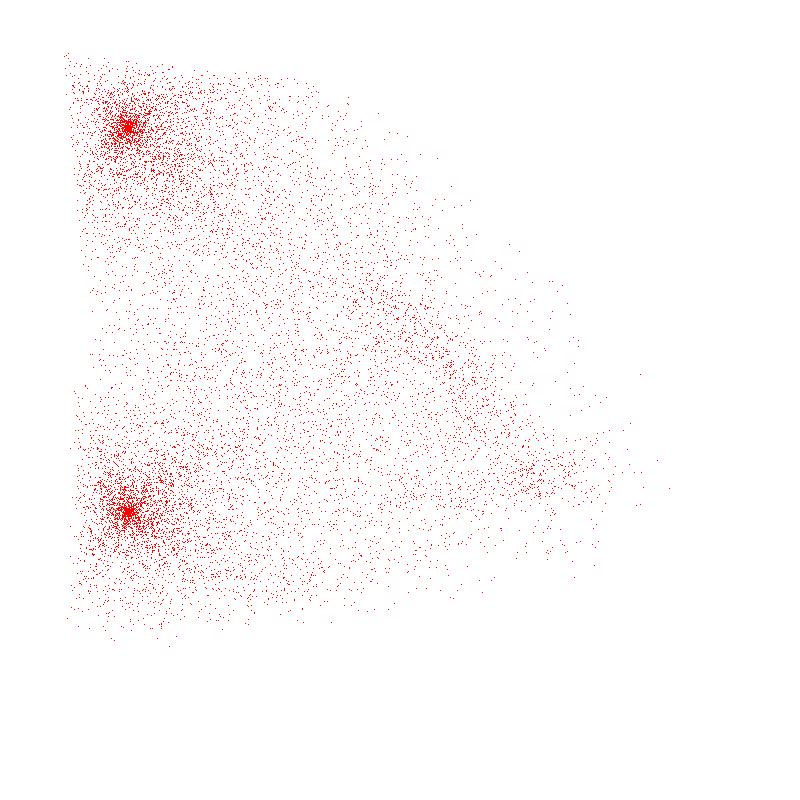
\includegraphics[width=84.5mm]{preview.png}
    \caption{Example frame of preview output (simple gravity system); approximately 15,000 particles}
    \label{fig:preview}
\end{figure}

The preview subsystem takes the output from the simulator and uses an OpenGL view to draw all of the particles as uniformly sized red dots, as you can see in figure \ref{fig:preview}. This rendering is very rough but also very quick --- fast enough to be real-time, in many cases.

Preview rendering should be used when designing particle systems, as it provides nearly instant --- though relatively unattractive --- feedback.

\subsection{Rendering}

Our renderer is currently very simple: it takes the particle data from the simulation phase and turns it into a greyscale image. It does this by iterating over each pixel of the output image, mapping the pixel's location into 'particle space', then searching through all of the particles, finding those which are within $\epsilon$ units of it, and updating the output image. Particles are orthographically projected onto the plane of the image, and --- at the moment --- depth information is completely ignored.

For the purposes of all of the systems contained in this paper, $\epsilon=0.1$.

There are two main rendering modes at the moment: {\bf smooth}, and {\bf cloudy}.

{\bf Cloudy} simply increments the luminance of the pixel for each particle it finds that's within $\epsilon$ units, leading to 'circles of influence' around each particle, as seen in figure \ref{titlefig}.

{\bf Smooth} weights the increase in luminance by the distance to the particle, according to $(0.1 - dist) \cdot 50$, as seen in figure \ref{smoothfig}.

We've asked numerous people which of the two rendering modes they prefer, and have come up almost completely split, so they're both included, for the time being.

\section{Performance \& Results}

\label{performanceSection}

\begin{figure}
    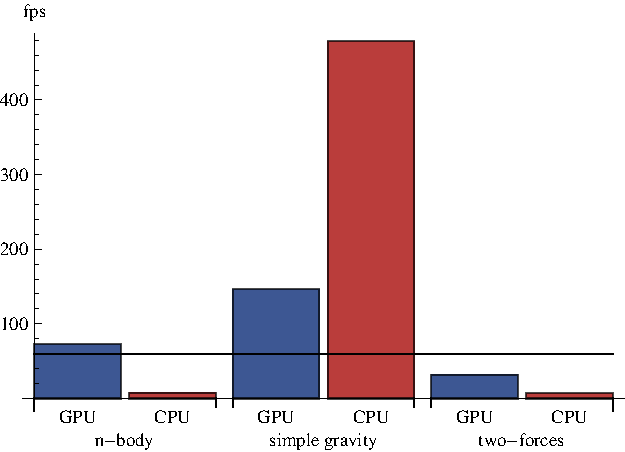
\includegraphics[width=84.5mm]{basicSpeedPlot.pdf}
    \caption{Simulation frame-rate of various different systems on CPU vs. GPU; higher values are better; the horizontal line rests at 60 fps}
    \label{fig:basicSpeedPlot}
\end{figure}

\subsection{Hardware}

All benchmarks and performance tests were taken on a machine running Mac OS X with a Core 2 Duo E7200 at 2$\times$2.53GHz with 8GB of RAM and an ATI Radeon 4890 at 800$\times$850MHz with 1GB of VRAM.

\subsection{Benchmarks}

Figure \ref{fig:basicSpeedPlot} shows the relative frame-rates of three different particle systems which we've been using as sample systems on the CPU versus the GPU.

The {\bf n-body} system is a simulation of 16,384 particles all interacting with each other, simulating gravity. There are no emitters in this system, and only one force.

The {\bf simple gravity} system (also pictured in figure \ref{titlefig}) is a simulation with two emitters --- which emit 20 particles per frame each --- and three equal-strength gravity wells (in the top right, top left, and center). The gravity simulation in this system is much simpler than in {\bf n-body}, as the particles don't interact with each other, just with the three wells.

The {\bf two-forces} system is a simulation with 1,048,576 particles and two outward-acting normal forces placed equidistant from the center on a diagonal through the random cloud of particles.

You'll note that {\bf n-body} shows a drastic speedup when moved to the GPU --- almost 10x! This is primarily because the n-body force is perfect for parallelization, as it has a long per-particle runtime (each particle has to iterate over all of the other particles, since we lack a spatial hashing data structure).

Something similar is true for {\bf two-forces}: while it's not actually nearly as computationally intensive per-particle, there are such a sheer number of particles that the parallelism comes into play in a big way, providing a less-impressive-but-still-significant 4$\times$ speedup.

The {\bf simple gravity} system shows the weakness of our approach: since emitters are evaluated on the CPU no matter what (because of the infeasbility of resizing buffers on the GPU discussed in section \ref{emitters}), and incur an additional pair of copies to/from the GPU, the CPU is able to significantly outpace the GPU. This makes it clear that emitter-heavy systems with few expensive forces are {\it not} well suited for our approach.

\subsection{Video}

Both the preview and rendering subsystems have the ability to output a PNG file for each simulated frame. These can be recombined and encoded with most video editing tools into a usable format.

\section{Applications}

\section{Future Work}

\subsection{Spatial Hashing}

One improvement which would massively improve the performance of both the renderer and some of the forces would be the inclusion of a spatial hashing mechanism.

For example, the renderer currently iterates over all of the particles to find the few which are very close to the pixel currently being rendered --- this operation is currently implemented in the most na\"{i}ve way possible, which is $O(n^2)$. The implementation of a kd-tree would make this $O(n^{2/3})$ instead --- quite a significant improvement, though at the expense of a measurable increase in complexity.

Alternatively, \cite{1281670}'s "force splatting" approach might make even better use of the optimized hardware available, though it's unclear to me that the summing operation (which their approach improves) is actually the primary bottleneck.

\subsection{Design Tools}

\subsection{Extended Properties}

\subsection{Rendering Improvements}

\subsection{Blender Integration}

\section{Conclusion}

\bibliographystyle{acmsiggraph}
\nocite{*}
\bibliography{report}

\end{document}